\section{Improved {\kvcache} cache system}
\label{sec:design}

\iffalse
\vspace{-1.ex}
\stitle{System requirements. }
As we have mentioned in the introduction, 
a {\kvcache} cache system has two requirements:
it should have high hit rate with minimized cache capacity. 
\fi

\subsection{An overview of the design space}
\label{sec:design-mechanism}

\noindent
Existing {\kvcache} cache systems~\cite{cachedattention, vllm,sglang,DBLP:journals/corr/abs-2403-14401}
follow similar caching mechanisms and policies.
Below we give a brief overview of their designs
before moving on to our improved policy. 


\stitle{Current {\kvcache} cache mechanism and policies. \,}
Regarding the mechanism:
existing systems cache {\kvcache}
primarily on GPU and CPU in a hierarchical manner.
The {\kvcache} is managed at block granularity (see \textsection{\ref{sec:bg}}):
when a {\kvcache} block is generated,
it is first cached on the GPU HBM.
If the GPU is unable to cache newly generated blocks due to out of memory,
the caching system adopts an eviction policy (described below)
to evict some blocks from the GPU to the CPU.
The evicted blocks are asynchronously swapped to CPU in a layer-by-layer manner
so the swap cost is negligible.
If the CPU is also out of memory,
the blocks are removed.
Before executing a new request,
if the request hits cached blocks,
the serving system directly reuses the cached blocks to avoid recomputation.
Note that if the hit is on CPU, the block is swapped to the GPU also in a layer-by-layer manner.

Regarding the policies: a {\kvcache} cache system mainly needs two policies:
how to determine cache hits and how to evict cached blocks.
For the first policy,
the design choices differ in their granularity of checking which blocks may contribute to the hits:
some systems check for matches across all requests~\cite{sglang,DBLP:journals/corr/abs-2404-12457}
while others only check for matches within requests from individual users~\cite{DBLP:journals/corr/abs-2403-14401, cachedattention}.
For the second policy,
current systems mainly adopt standard eviction policies like LRU or FIFO.
Though they adopt some extensions
like checking whether the evicted blocks are in the scheduling queue~\cite{cachedattention},
the overall rationale does not change.

\stitle{The drawback. \,}
Existing workload-agnostic policies
like LRU may miss the workload features we analyzed in \textsection{\ref{sec:analyze}},
and we argue that they are suboptimal.
Take Trace A as an example:
given the same amount of time since the last access (e.g., greater than 10 seconds),
10-turn text requests are more likely to have a subsequent turn than 1-turn text requests
(see {\fig{fig:motiv-next-turn-probability}}).
However, if many 1-turn requests are flooding into the system,
10-turn requests can be evicted by LRU
because the reuse time is longer.

\iffalse
Second, there lacks an accurate estimator for {\kvcache} capacity requirements based on workload patterns. 
Naively adopting a deep GPU-CPU-SSD cache hierarchy would waste storage resources. 
For example, under CachedAttention~\cite{cachedattention}'s setup, 
memory would be underutilized before reaching an ideal cache hit rate, 
as we will discuss further in \textsection{\ref{sec:design-eval}}. 
\fi

\iffalse
\stitle{Our solution: workload-aware eviction policy.}
To this end, we propose a workload-aware cache eviction policy 
that considers the predictable reuse time and next-turn probability
of each request type,
based on our characterizations described in \textsection{\ref{sec:motiv-temporal-spatial}}. 
We follow the mechanisms of existing {\kvcache} cache systems~\cite{cachedattention, vllm,sglang,DBLP:journals/corr/abs-2403-14401}---including
asynchronous swapping and pipelined loading, 
as they are workload-independent and have converged to a similar design. 
Note that our characterization can potentially open more opportunities 
for more improved system designs. 
For example, given that cross-user cache hits are rare (see {\fig{fig:motiv-cross-hit}}), 
we can accelerate the checking process by implementing per-user prefix checks. 
%Some existing systems have already adopted this approach~\cite{cachedattention,DBLP:journals/corr/abs-2403-14401}.
We leave a deeper exploration as our future work. 
\fi


\begin{table}[!t]
    \centering
%    \vspace{2.2mm}
    \small{
        \resizebox{1\linewidth}{!}{
            \ra{1.2}
\begin{tabular}{@{}p{0.45\linewidth}p{0.45\linewidth}@{}} \toprule
\textbf{Observations}                                                                                    & \textbf{Techniques}                                                      \\ \hline
The probability of {\kvcache} reuse follows exponential distributions given a workload 
({\fig{fig:motiv-next-turn-probability}} and {\fig{fig:motiv-reuse-time-probability-hist}}). 
& \ding{192} Workload-aware reuse-probability-distribution-based priority estimation.                   \\

Spatial locality ({\fig{fig:motiv-spatial}}--\ref{fig:motiv-spatial-workload}).                                                                                        
& \ding{193} Assign a higher priority to the head {\kvcache} blocks. \\

Ephemeral {\kvcache} lifespan ({\fig{fig:motiv-block-timespan}}).                                                          
& \ding{194} Remove frequency when calculating the priority,
as well as limiting the time span of probability calculation.                                     \\
\bottomrule
\end{tabular}
            
        }
    } \\[8pt]
    \begin{minipage}{1\linewidth}
        \caption{\small{\emph{
        A summary of the main techniques in our workload-aware cache eviction policy
        based on the findings in \textsection{\ref{sec:analyze}} 
        }}}
    \label{tab:insights}
    \end{minipage} \\[-5pt]
\end{table}  


\iffalse
\begin{table}[t]
\centering
\caption{Key Insights and Technical Realizations for {\kvcache} Policy Design}
\label{tab:policy-insights}
\begin{tabular}{@{}p{0.45\linewidth}p{0.45\linewidth}@{}}
\toprule
\textbf{Key Insight} & \textbf{Technical Realization} \\
\midrule
equal importance single/multi-turn requests & 
Different scenarios (e.g., Trace A and Trace B) can use different policies  \\
\midrule
% Multi-turn requests have high variability. The probability of issuing the next turn request is predictable given a workload category. Different workload types have distinct {\kvcache} temporal locality and short reuse time.
% The reuse probability distributions of individual workload categories are statistically predictable and exhibit significant heterogeneity across categories. & 
predictable reuse distributions with cross-category heterogeneity & 
Workload-aware policies (e.g., fitting exponential distributions per workload)  \\
\midrule
spatial locality & 
Consider size (prefix length) in policy  \\
\midrule
ephemeral {\kvcache} lifespan & 
Finite time reuse over LFU to prevent dead-cache buildup \\
\bottomrule
\end{tabular}
\end{table}
\fi

\stitle{Our solution: workload-aware reuse-probability-distribution-based {\kvcache} eviction policy. \,}
To this end, we propose a workload-aware cache eviction policy
that considers the reuse probability distributions
of each request category based on the characterizations
presented in \textsection{\ref{sec:motiv-temporal-spatial}}.
At a high level, at the eviction time, 
for each block, we calculate a priority---the likelihood of a {\kvcache} being reused
in the future based on the profiled reuse probability distribution 
of its request category (workload).
The priority further holistically considers the spatial locality as well as
the short lifespan of {\kvcache} blocks.
The blocks with the lowest priority are evicted first.
Table~\ref{tab:insights} summarizes our techniques
as well as their corresponding observations from \textsection{\ref{sec:analyze}}.

Our caching mechanisms follow 
existing systems~\cite{cachedattention, vllm, sglang, DBLP:journals/corr/abs-2403-14401}---including
asynchronous swapping and pipelined loading,
as these techniques have converged to a standard design. 


\subsection{Workload-aware {\kvcache} cache eviction policy}
\label{sec:design-policy}

%\nospacestitle{Deriving the priority {\kvcache} blocks with its workload reuse probability. \,}
\nospacestitle{Existing workload-aware policy. \,}
Workload-aware cache eviction policy has been extensively studied in the literature~\cite{cherkasova1998improving,lruk,slru,lirs,arc,lhd,cacheus}.
A representative policy is the Greedy-Dual-Frequency-Size (GDFS) policy~\cite{cherkasova1998improving}, 
which evaluates the priority of each cached object (e.g., {\kvcache}) 
using the following workload-dependent features: 
$$
\text{Priority} = \text{Clock} + \frac{\text{Frequency} \times \text{Cost}}{\text{Size}}\,(\text{\uline{Existing GDFS}})
$$
The \texttt{Clock} captures the last access time of an object (similar to LRU),
the \texttt{Frequency} is the total access count of an object (similar to LFU),
the \texttt{Size} is the size of the cached object,
and \texttt{Cost} is the cost to bring the cached content back to the cache.
Objects with the lowest priority are evicted first.

\iffalse
As shown in \tbl{tab:policy-insights}, we will find that since
single-turn and multi-turns requests are equally important under different traces,
we can use different cache policy for different scenarios
(As evaluated in {\fig{fig:eval-qwen7b-cpu-cache}}--{\fig{fig:eval-llama70b-cpu-cache}}).
And considering the predictable and heterogeneous reuse distirbutions, we will add
a workload-aware mechanism to calculate {\kvcache} block priority for different workloads.
Besides the priority, we will consider prefix length under the same priority.
Finally, we remove the frequency from GDFS due to the ephemeral {\kvcache} lifespan,
LFU will easily cause the dead {\kvcache} block heap up to hinder the new cache.
\fi

\iffalse
As demonstrated in {\tbl{tab:policy-insights}}, our analysis reveals that
single-turn and multi-turn request patterns exhibit comparable significance
across diverse workloads.
This insight motivates the adoption of adaptive cache policies tailored to
distinct operational scenarios, as empirically validated in
{\fig{fig:eval-qwen7b-cpu-cache}}--{\fig{fig:eval-llama70b-cpu-cache}}.
Furthermore, the observed predictable yet heterogeneous reuse distributions
across workloads necessitate a workload-aware prioritization mechanism for {\kvcache} blocks.
While prioritizing blocks, we further incorporate prefix length as a secondary discriminant
under equivalent priority levels to optimize cache utilization.
Notably, we exclude the frequency metric from the GDFS algorithm due to
the transient nature of {\kvcache} blocks. As shown in our evaluations,
retaining frequency-based metrics (such as those employed in the LFU policy) introduces
the risk of obsolete cache entries accumulating and displacing higher-value,
newly generated blocks.
\fi

While the above GDFS formulation can be retrofitted for calculating the priority of {\kvcache} blocks,
we found it does not fully consider the {\kvcache} usage in LLM serving
as well as the known probability distributions of requests in different categories.
For example, a frequently accessed block may not be reused in the future due to the short lifespan of {\kvcache} blocks,
causing a frequently accessed then died block wasting the {\kvcache} space.
Besides, a block with higher cost to bring to the cache
does not necessarily mean it is more likely to be reused in the future.
Instead, we need to bring the more likely to be reused blocks to the cache first.
While such workload information is not available in the setup of GDFS,
it is readily available in serving LLMs based on our characterization in the previous section.

\begin{figure}[!t]
    \begin{minipage}{.9\linewidth}
    \hspace{4mm}
%    \centering    
    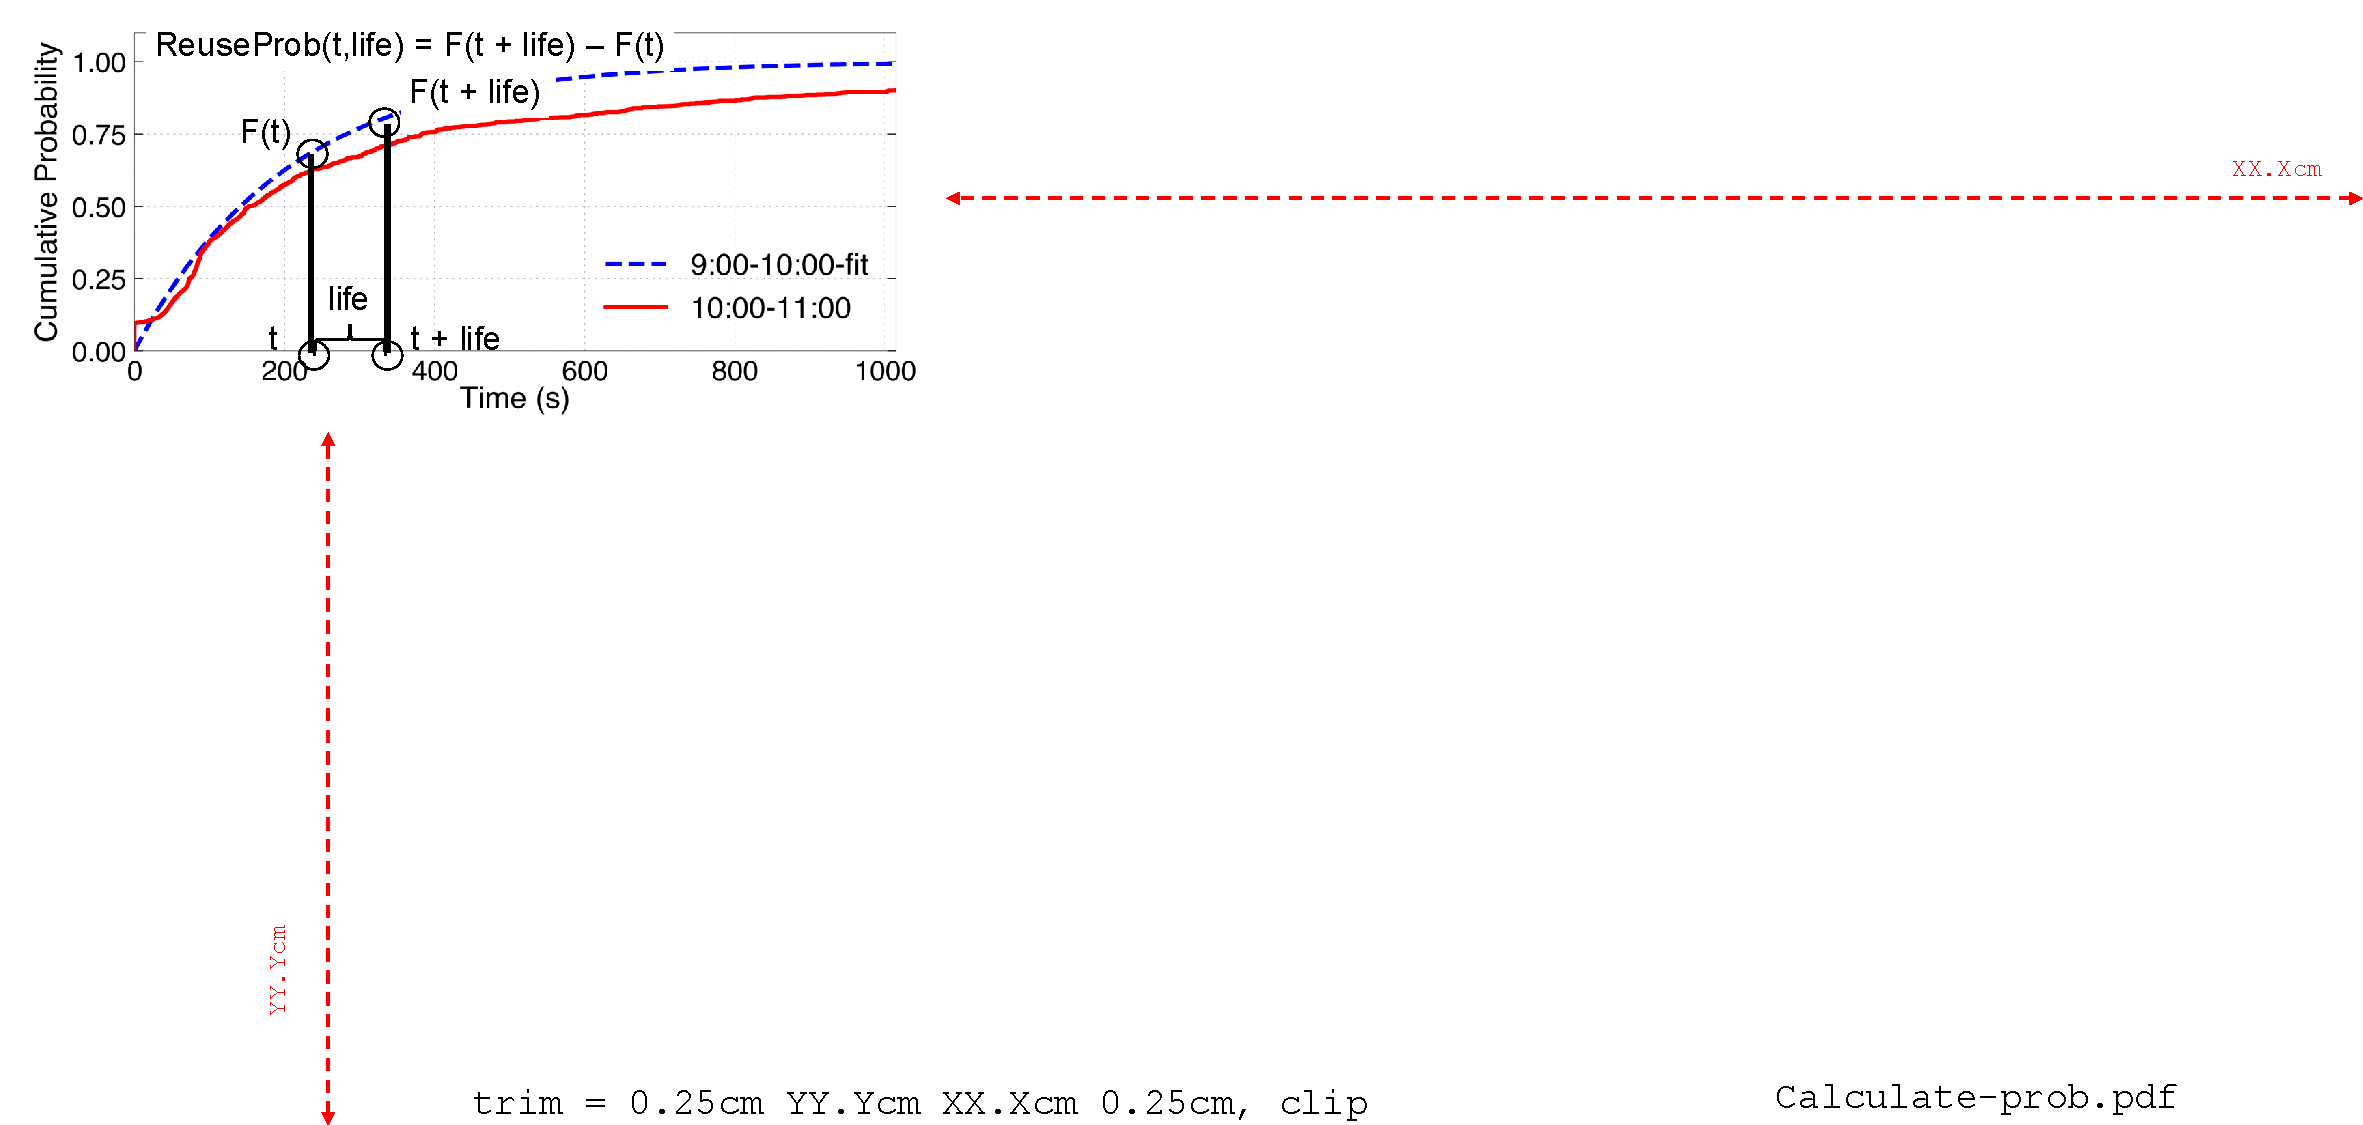
\includegraphics[width=1\textwidth, trim=0.25cm 11.8cm 24cm 0.25cm, clip]{figs/calculate-prob.pdf} 
    \end{minipage} \\[0pt]
    \begin{minipage}{1\linewidth}
    \caption{\small{\textit{
        An illustration of how to calculate the reuse probability of a {\kvcache} block
        given its workload (request category). 
    }}}
    \label{fig:example-request-category}
    \end{minipage} \\[-15pt]
\end{figure}

\stitle{Our policy. \,}
We follow GDFS to calculate the priority of each {\kvcache} block and use
the priority to determine the eviction order,
but our priority is retrofitted with our characterized {\kvcache} reuse features:
$$
\text{Priority} = ({\text{ReuseProb}_w(t, \text{life})},{-\text{Offset}}) \,(\text{\uline{Workload-aware}})
$$
\noindent
Specifically, the priority is represented with a tuple containing two metrics
and we compare the tuple with lexicographical order.
The rationale behind the two metrics is: \\[-10pt]
\begin{itemize}[leftmargin=*,leftmargin=10pt,itemindent=0pt]
    \item \textbf{ReuseProb$_w$} (\ding{192}) calculates the reuse probability of a {\kvcache} block
    at a given time $t$, where $t$ means the time since its last access.
    For each workload (request category),
    the reuse probability is calculated using a two-step process.
    First, we sample a period of the recently accessed data in the background.
    Second, based on the observations in {\fig{fig:motiv-reuse-time-probability-hist}},
    we fit an exponential distribution to the sampled data,
    and look up the fitted curve to get the reuse probability.
    {\fig{fig:example-request-category}} shows an example of how to calculate the reuse probability.
    We first use the background sampled data from 9:00 a.m. to 10:00 a.m. to fit the cumulative distribution function (CDF) of the
    reuse probability of a given workload (blue line).

    Note that the fitted curve is close to the real data (red line).
    Afterward, we can look up the curve to get the reuse probability of a {\kvcache} block in the future.
    Note that the function further considers the expected lifespan (life) of the block,
    which is critical considering the short lifespan of {\kvcache} and we describe below.  \\[-10pt]

    \item \textbf{Offset} (\ding{193}) considers the spatial locality described in 
    \textsection{\ref{sec:motiv-temporal-spatial}}:
    the priority is reversely proportional to the prefix length of the {\kvcache} block in the entire request. \\[-10pt]
\end{itemize}

We don't consider frequency explicitly  (\ding{194})
because we found it can not provide useful information for cache policy
due to the short lifespan of {\kvcache} blocks (see {\fig{fig:motiv-block-timespan}}) even for frequently reused ones.
More importantly, we also need to regulate the calculated reuse probability
with the lifespan.
If not, the fitted reuse probability will return a large probability for a request
with long-tailed reuse time distribution for a long time.
This contradicts the short {\kvcache} lifespan observation
and leads to the inefficient utilization of limited cache space.


\iffalse
As shown in {\fig{fig:motiv-reuse-time-probability-multiline}},
different workloads exhibit distinct reuse probability distributions.
However, each workload maintains a relatively stable probability distribution
over extended periods (e.g., peak hours between 9 a.m. and 11 a.m.).
Thus, we leverage trace data from the preceding hour to predict the
reuse probability distribution for the subsequent hour for each workload.
% \fig{fig:motiv-reuse-time-probability-hist} further demonstrates that
each workload’s reuse distribution closely approximates an exponential distribution.
Consequently, we derive a fitting coefficient $\lambda_w$
for each workload $w$ based on the trace data collected over the past hour.
Within the same monitoring window, we also compute the block reuse probability $p_w$
for each workload’s {\kvcache} block. Combining these parameters,
the reuse probability density function for workload $w$ is formulated as:
$$
f_w(t) = p_w \cdot \lambda_w e^{-\lambda_w t}
$$
where $t$ denotes the time elapsed since the last access
(i.e., $t = \text{current\_time} - \text{last\_accessed\_time}$).

Now, for each workload's {\kvcache} block with a and workload category $w$,
For a {\kvcache} block belonging to workload $w$ with a last access time $\text{last\_accessed\_time}_b$,
its reuse probability at the current time $t_0$
is calculated by integrating the distribution function over the interval
$[t_0 - \text{last\_accessed\_time}_b, +\infty)$:
$$
p_b = \int_{t_0 - \text{last\_accessed\_time}_b}^{+\infty} p_w \cdot \lambda_w e^{-\lambda_w t} \mathrm{d}t
$$

For each {\kvcache} block, we compute its reuse probability and prioritize eviction
of the block with the lowest reuse probability (i.e., minimal priority),
as outlined in {\alg{alg:naive-eviction}}.

Our policy further incorporates prefix awareness, prioritizing eviction of blocks
corresponding to later segments of input or output sequences. This design stems from
the observation that prefix blocks within the same request exhibit stronger
reuse likelihood (see spatial locality analysis in \textsection{\ref{sec:motiv-temporal-spatial}}).
Implementing this is straightforward: for blocks sharing the same minimal priority,
we compare their size (i.e., the number of prefix tokens) and select the block with
the largest size for eviction.

While our policy is conceptually inspired by GDFS, it currently omits explicit cost modeling.
Unlike GDFS, which defines cost as the resource overhead of cache re-accesses, we define
the cost for {\kvcache} blocks as the opportunity cost of retaining them in memory until reuse.
Specifically, since all {\kvcache} blocks incur identical recomputation costs during prefill,
we focus on temporal efficiency: the duration a block occupies cache space before potential reuse.
Calculating reuse probability over an infinite future horizon risks retaining blocks with
long-tailed reuse distributions for disproportionately extended periods to realize marginal
reuse gains. This inflates opportunity costs by displacing higher-value blocks.
To mitigate this, we introduce a finite time range for reuse probability computation:
$$
p_b = \int_{t_0 - \text{last\_accessed\_time}_b}^{t_0 - \text{last\_accessed\_time}_b + \text{time\_span}} p_w \cdot \lambda_w e^{-\lambda_w t} \mathrm{d}t
$$
The $\text{time\_span}$ is determined by cache capacity constraints and workload characteristics:
$$
\text{time\_span} = \frac{M \cdot \text{block\_size}}{\text{QPS} \cdot \text{mean\_sequence\_length}}
$$
where $M$ denotes the total number of {\kvcache} blocks that fit within the cache capacity.
This formulation ensures the time range corresponds to the duration required to refresh
the entire cache space with new blocks under current workload
conditions (e.g., query rate and sequence length statistics).
\fi

\iffalse
We have noticed that there is a larger kvcache reuse interval time in traceA.
When the kvcache memory space is limited, especially in model with MHA, many kvcache have no chance to reuse
before they are evicted. In the traditional cache policy, new generated kvcache always have bigger priority to
stay in the cache memory. But from the trace analysis, we claim that different workload types and chat under
different turn have the different opportunities to be reused. So we set a monitor for the long running system
which will have a stable reuse probability and reuse time for different workloads and differnet turns on average.
For each workload type and chat turn, our monitor has a average reuse probability $P_w$ and average reuse time $T_w$ for it.
Meanwhile, we will maintain a P90 reuse time $T^{90}_w$ for it.
And under a continuous time like 10 minutes, the system load is ralative stable. So we can use last 5 minutes
system load to represent the system load in the future 5 minutes. We define the system load as the total
input and output tokens in the last 5 minutes. So we can get the system load for a unit time as $L$.
Then we can define the priority for a request with input prompt length $L_p$ as:
\fi

\iffalse
We start with a brief review of the original GDFS method and then move on to our extensions. 
Specifically, GDFS evaluates the priority of each cached object, 
i.e., a {\kvcache} block in our setup
based on its accessed time, frequency, size and access cost,
whose priority is defined as follows: 
$$
P_w = \text{Clock} + \frac{\text{Frequency} \times \text{Cost}_w}{\text{Size}}
$$
\noindent
\texttt{Clock} captures the recency of execution, which is updated upon eviction. 
If a block is reused, its clock is set to ensure that an unused block has a smaller clock. 
\texttt{Frequency} is the total access count of a block in a time window. 
\texttt{Size} is the number of tokens in a block. 
\texttt{Cost} is the cost to bring the cached content back to the cache. 
In the GDFS method, the cached blocks with lower priorities are first evicted. 

Naively reusing the GDFS is non-optimal 
because it doesn't consider the predictable workload features 
like reuse time and reuse probability. 
We extend the \texttt{Cost} to further consider these factors. 
Since the reuse time and probability are relatively predictable given a workload category,
we parameterize the priority based on the workload type $w$, 
where $\text{Cost}_w$ is defined as follows: 
$$
\text{Cost}_w = \frac{P_w}{T_w}
$$
\noindent
Note that the workload category considers both the request type as well 
as the current turn of the request. 
$P_w$ is the predicated probability that the category generating the block 
will engage in the next-turn request, 
and $T_w$ is the predicated reuse time for the request. 
Intuitively, the priority is proportional to the probability to start the next turn, 
and the requests with shorter reuse time is prioritized. 
Since the serving system knows the request category after receiving each request, 
we can profile both metrics during runtime. 

Besides the workload-awareness, our {\policy} is also prefix-aware, 
meaning that blocks that corresponding to the later part of the input and output 
are evicted first. 
This is because for the {\kvcache} blocks belonging to the same request, 
the prefix blocks are likely to be reused (see the spatial locality analysis in \textsection{\ref{sec:motiv-temporal-spatial}}).
Achieving so is trivial: 
since all the blocks in the same request will have the same priority based on our definition,
before eviction, we will examine all the blocks with the same priority,
sort them with the prefix, and then do the eviction.
\fi

\iffalse
\begin{algorithm}[!t]
    \caption{\emph{Naive Cache Block Eviction Algorithm}} \label{alg:naive-eviction}
    \SetAlgoLined
    \KwInput{ 
        $\bf{Bs}$ is the set of cache blocks.
        $\bf{TimeRange}$ is the range for probability calculation.
        $\bf{\Lambda}$ is the set of workloads' exponential distribution fitting coefficients.
        $\bf{P}$ is the set of workloads' cache block reuse probabilities.
        $\bf{\Lambda}$ and $\bf{P}$ are updated by the monitor periodically.
    }
    \KwOutput{The evicted cache block $\mathbf{B}$}

    $\text{CurT} \gets \text{time.time()}$

    $\text{MinPriority} \gets +\infty$

    $\text{ChosenBlock} \gets \text{None}$

    \For{$b \in Bs$} {
        $\text{Priority} \gets \text{GetReuseProb}(b, \text{CurT}, \text{TimeRange}, \Lambda, P)$

        \If{$\text{Priority} < \text{MinPriority}$} {
            $\text{MinPriority} \gets \text{Priority}$

            $\text{ChosenBlock} \gets b$
        }
    }

    $\text{B} \gets \text{ChosenBlock}$

    \Return $\text{B}$
\end{algorithm}
\fi

\begin{figure}[!t]
    \begin{minipage}{1\linewidth}
    \hspace{-1mm}
    \centering    
    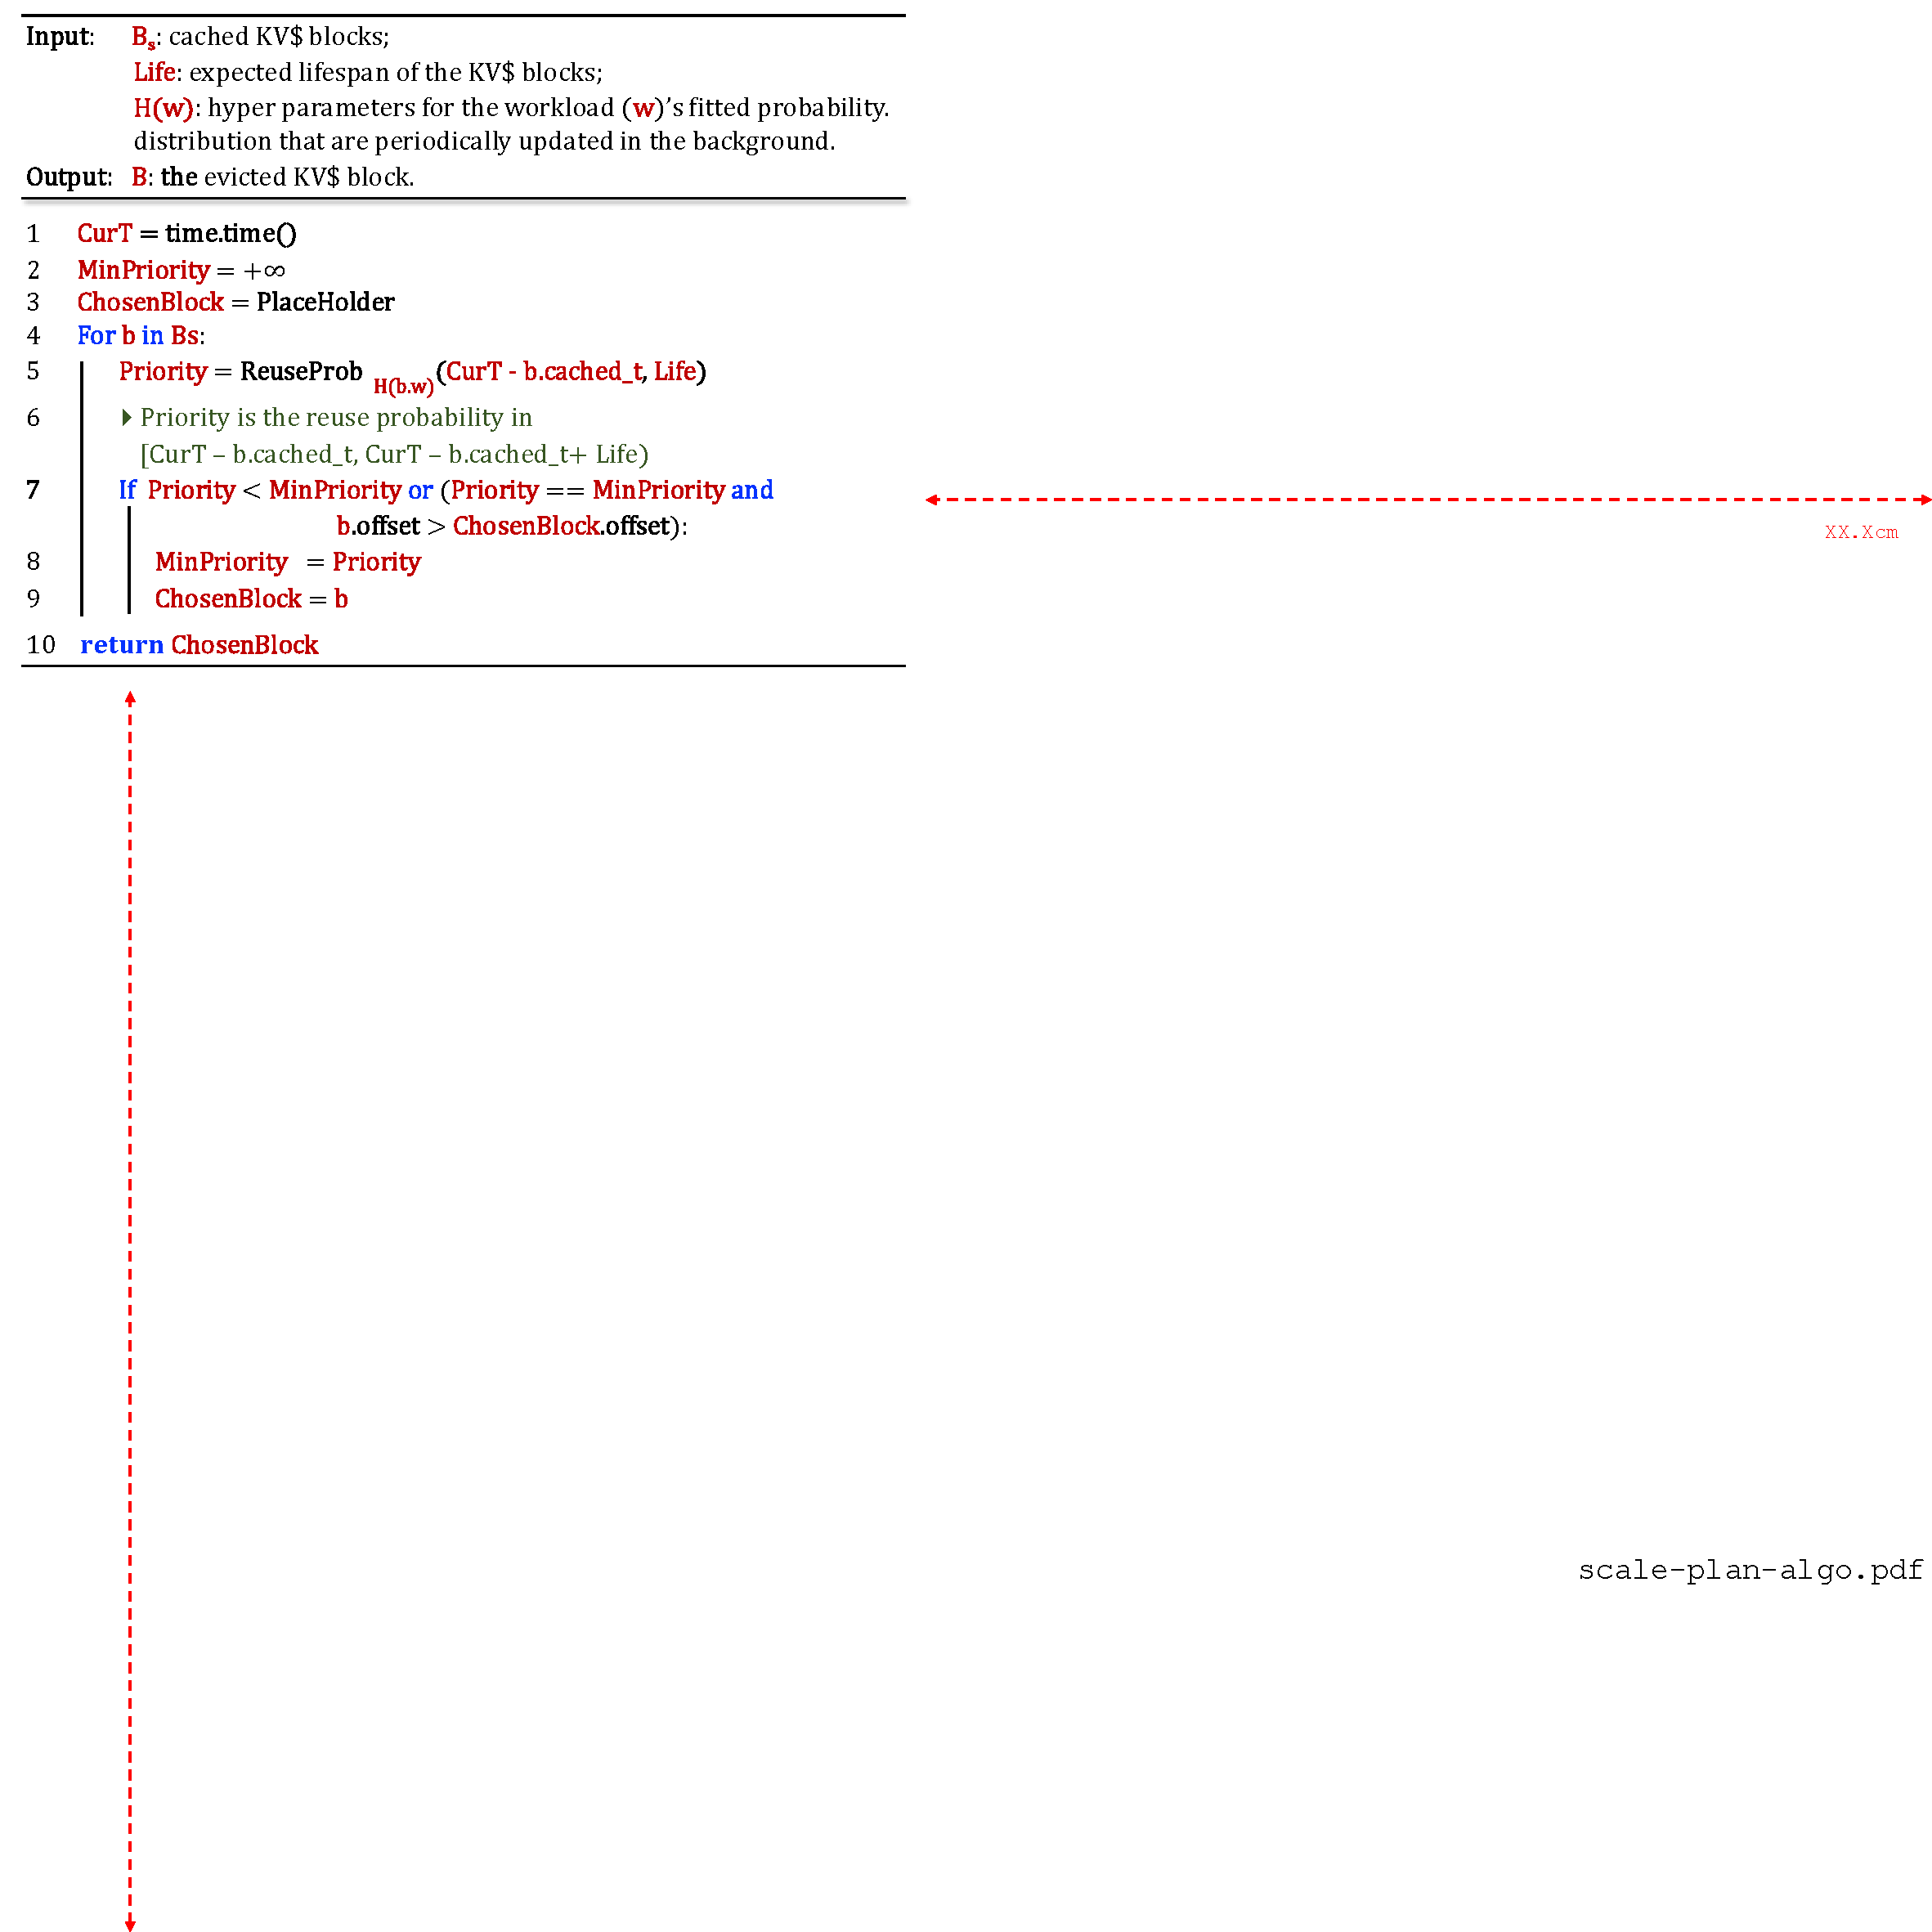
\includegraphics[width=1\textwidth, trim=0.25cm 25.8cm 21cm 0.25cm, clip]{figs/naive-eviction-algo.pdf} 
    \end{minipage} \\[4pt]
    \begin{minipage}{1\linewidth}
    \caption{\small{\textit{
        A simplified pseudocode of our workload-aware cache eviction algorithm.
    }}}
    \label{alg:naive-eviction}
    \end{minipage} \\[-5pt]
\end{figure}

\stitle{The detailed eviction algorithm. \,}
Algorithm~\ref{alg:naive-eviction} presents a simplified pseudocode of our workload-aware cache eviction algorithm.
Upon eviction,
we first iterate through all the cached blocks (line 4--6)
and calculate the reuse probability for each block using the workload ($b.w$).
The priority is then compared with the offset of the block
to update the block to be evicted (line 7--9).

\stitle{Performance optimization. \,}
One drawback of the above naive algorithm is that it
requires computing the reuse probabilities of all {\kvcache} blocks to identify the least reusable candidate.
To avoid excessive computation overhead,
we observe that all {\kvcache} blocks
within each workload are naturally ordered by their last accessed timestamps according to the exponential distribution,
so we can avoid computing the reuse probability when comparing blocks within the same workload.
Specifically, for each workload, we maintain
a priority queue of its {\kvcache} blocks ordered by last accessed time.
During eviction, instead of scanning all blocks, we first treat the least-recently-used block
of each workload as the candidate for eviction.
Afterward, we run the algorithm described in Algorithm~\ref{alg:naive-eviction}
to obtain the final evicted block.
This reduces the complexity from $O(N)$ to $O(W)$,
where $W$ is the number of workloads (typically in the range of tens).
As a result, the performance overhead of workload-aware policy is negligible to serving,
e.g., we observed a 79\,$\mu$s policy delay for each eviction,
with the aggregated overhead only 1.2\,\% of the scheduling overhead 
of a typical serving engine (vLLM~\cite{vllm}). 

\iffalse
\begin{algorithm}[!t]
    \caption{\emph{Cache Block Eviction Algorithm}} \label{alg:eviction}
    \SetAlgoLined
    \KwInput{ 
        $\bf{W_{pq}}$ is the set of workload min priority queues organized by their last_accessed_time.
        $\bf{TimeRange}$ is the range for probability calculation.
        $\bf{\Lambda}$ is the set of workloads' exponential distribution fitting coefficients.
        $\bf{P}$ is the set of workloads' cache block reuse probabilities.
    }
    \KwOutput{The evicted cache block $\mathbf{B}$}

    $\text{CurrentTime} \gets \text{time.time()}$

    $\text{MinPriority} \gets +\infty$

    $\text{ChosenW} \gets \text{None}$

    \For{$(w, pq) \in W_{pq}$} {
        \Comment{$w$ is one of the workload in the workload set, $pq$ is the corresponding priority queue for this workload.}

        $\text{b} \gets pq.\text{top()}.\text{LastAccessedTime}$

        $\text{Priority} \gets \text{GetReuseProb}(b, \text{CurT}, \text{TimeRange}, \Lambda, P)$

        \Comment{Priority is the reuse probability in $[\text{CurrentTime} - \text{T}, \text{CurrentTime} - \text{T} + \text{TimeRange}]$}

        \If{$\text{Priority} < \text{MinPriority}$} {
            $\text{MinPriority} \gets \text{Priority}$

            $\text{ChosenW} \gets w$
        }
    }

    $\text{B} \gets W_{pq}[\text{ChosenW}].\text{pop()}$

    \Return $\text{B}$
\end{algorithm}
\fi

\iffalse
\begin{figure}[!t]
    \begin{minipage}{1\linewidth}
    \hspace{-1mm}
    \centering    
    \includegraphics[width=1\textwidth, trim=0.25cm 23.0cm 21cm 0.25cm, clip]{figs/eviction-algo.pdf} \\[1pt]
    \end{minipage} \\[3pt]
    \begin{minipage}{1\linewidth}
    \caption{\small{\textit{
        The pseudocode of the cache eviction algorithm.
    }}}
    \label{alg:eviction}
    \end{minipage} \\[-15pt]
\end{figure}

\stitle{Workload monitoring. }
We extend the scheduler to timely monitor the patterns of different 
workload categories. 
Collecting such metrics has negligible overheads 
because 
the additional metadata to track as well as the collection overhead is small. 
For example, 
vllm~\cite{vllm} already has a \texttt{last\_accessed\_time} 
for each cached block
such that we can use to calculate the reuse time. 
Besides, there are only dozens of request categories even considering the request turns.
\fi

\iffalse
\subsection{Workload-aware cache capacity predicator}
\label{sec:design-predicator}

We found that the activate {\kvcache} block capacity to reach the ideal cache rate is predictable thanks to the
stable {\kvcache} timespan of different workloads. We design a predicator to capture
the cache capacity to reach the ideal cache hit rate based the characterization of 
workloads.

Our predicator maintains the priority for all {\kvcache} blocks in the serving system.
The higher priority means the higher possibility to be reused in the future. If the priority
of a block exceeds a \emph{threshold}, our predicator will treat this block as 
Our predicator is based on three observations about the workload.

First, considering the skewed workload distribution in both to-B and to-C workloads, we 
use a factor $w(type)$ to indicate the weight for each workload type, the
weight factor is updated dynamically during the serving process.

Second, since most block reuse time is relative short, our predicator will decrease the
block priority if the block is too staled. For example, in traceA, more than 95\% percent 
blocks are never used again after 561 seconds, our predicator will decrease the priority of
these blocks.

Third, since the kv-cache blocks that are closer to the front are more likely to be hit, 
our predictor will set the initial priorities of all blocks of a request in decreasing order.
\fi


\subsection{Performance evaluation}
\label{sec:design-eval}

\nospacestitle{Testbed. \,}
We conducted our evaluations on a server with 8 NVIDIA A800-80GB GPUs.
The GPUs are connected via 400\,GBps bidirectional NVLink, 
allowing us to use multiple GPUs (e.g., 4) to serve a single large model
with tensor parallelism~\cite{narayanan2021efficient}. 
The GPUs are connected to the host via PCIe Gen4, 
offering a bidirectional bandwidth of up to 32\,GBps
between GPU HBM and the host memory. 


\stitle{Implementations and baselines. \,}
Since the state-of-the-art {\kvcache} cache systems that
incorporate both CPU and GPU {\kvcache} like
CachedAttention~\cite{cachedattention} and Pensieve~\cite{DBLP:journals/corr/abs-2403-14401}
are not open-sourced,
we implement a CPU-GPU {\kvcache} cache on vLLM~\cite{vllm},
the state-of-the-art LLM serving system that adopts GPU {\kvcache} cache by default.
We have further integrated the policies and mechanisms from state-of-the-art
(see \textsection{\ref{sec:design-mechanism}}) to it.
We have calibrated that
our implementation has a similar performance to state-of-the-art like CachedAttention
on the same synthetic workload with a similar testbed.

Besides integrating a CPU {\kvcache} cache on vLLM,
we have also implemented the {\kvcache}-centric global scheduler described in Mooncake~\cite{mooncake},
because serving LLMs on multiple instances is common. 
Specifically, the global scheduler will record the global {\kvcache} cache usage
and schedule the request to the instance with cached {\kvcache} whenever possible. 
Note that our workload-aware caching policy only applies to a single serving instance,
extending it to a global layer is left as our future work. 

\stitle{Evaluated models and workloads. \,}
We use three representative open-source models for the performance evaluations: 
Qwen2-7B~\cite{qwen}, 
Llama2-13B~\cite{llama2} and Llama3-70B~\cite{DBLP:journals/corr/abs-2407-21783}.
The rationale for choosing these models and the differences between them have been 
discussed in the per-request {\kvcache} size analysis in \textsection{\ref{sec:analyze-capacity}}. 
For Qwen2-7B and Llama2-13B models, we use one GPU per serving instance. 
For Llama3-70B, we use 4 GPUs. 
We use the Trace A and B described in \textsection{\ref{sec:workload-data}} as our evaluated workloads. 
Since we don't have sufficient GPUs to support the real workload,
we scale the traces to fit the processing capability of our testbed
using the scaling method that preserves the temporal pattern of the trace~\cite{DBLP:conf/eurosys/SajalHZU021}. 

\stitle{Evaluation methodology on anonymous traces. \,}
Even though the traces are anonymous,
we can evaluate the system serving performance
by constructing inputs that accurately reproduce the original trace's cache hit patterns.
Specifically,
for each anonymous block without assigned tokens,
we randomly generate a token list, ensuring each generated list's hash differs from all other token lists.
Moreover, to match the original input's iteration count,
we constrain the model using the trace's output length.
Finally, we replace the model-generated output with the constructed tokens
to preserve the cache patterns of multi-turn requests.


\iffalse
\begin{figure}[!t]
    %\hspace{-3mm}
    \centering
    \includegraphics[width=1.0\linewidth,center]{./data/qwen7b-vllm\figsuffix}  \\[1pt]
    \begin{minipage}{1\linewidth}
    \caption{\small{\emph{        
        {\kvcache} cache hit rate and LLM serving performance on Qwen2-7B. 
    }}}
    \label{fig:eval-qwen7b}
    \end{minipage} \\[-5pt]
\end{figure} 

\begin{figure}[!t]
    %\hspace{-3mm}
    \centering
    \includegraphics[width=1.0\linewidth,center]{./data/llama13b-vllm\figsuffix}  \\[1pt]
    \begin{minipage}{1\linewidth}
    \caption{\small{\emph{        
        {\kvcache} cache hit rate and LLM serving performance on Llama2-13B. 
    }}}
    \label{fig:eval-llama13b}
    \end{minipage} \\[-5pt]
\end{figure} 

\begin{figure}[!t]
    %\hspace{-3mm}
    \centering
    \includegraphics[width=1.0\linewidth,center]{./data/llama70b-vllm\figsuffix}  \\[1pt]
    \begin{minipage}{1\linewidth}
    \caption{\small{\emph{        
        {\kvcache} cache hit rate and LLM serving performance on Llama3-70B. 
    }}}
    \label{fig:eval-llama70b}
    \end{minipage} \\[-5pt]
\end{figure} 
\fi

\iffalse
\stitle{Overall performance. }
{\fig{fig:eval-qwen7b}}, {\fig{fig:eval-llama13b}} and {\fig{fig:eval-llama70b}} 
show the cache hit rate as well as throughput vs. latency graphs for three models. 
We report the serving latency as the queued time-to-first-token (QTTFT),
which includes both the model computation time and the queuing time. 
The throughput vs. latency graph is drawn by 
increasing the requests sent to each serving instance. 
For policies other than our {\policy}, 
they only use GPU for caching since it is the default setup in vllm. 
We analyze the effect of our policy on GPU-CPU caching in the next experiment. 

We can draw the following observations.
First, 
{\kvcache} cache can benefit LLM serving workloads: 
the throughput of vllm (+CPU {\policy}) is up to 22\%, 10\% and 30\%
higher than vllm without caching on two traces for model Qwen2-7B, Llama2-13B and Llama3-70B.
Second, a higher cache hit ratio typically implies better performance, 
but the improved ratio depends on the models evaluated. 
For Qwen2-7B and Llama2-13B, under high throughput they are bottlenecked by the decode phase of LLM,
which is memory bound~\cite{DBLP:conf/osdi/ZhongLCHZL0024,DBLP:conf/isca/PatelCZSGMB24},
so the saved computation of {\kvcache} cache is less effective. 
For example, when increasing 33.2\% and 11.3\% hit rate with our {\policy} (+CPU), 
the throughput of vllm only increase by 4\% and 2\% on Trace A and Trace B for Qwen2-7B, respectively.
In comparison, Llama3-70B is computation bound due to its huge parameter size,
so a 16.3\% and 9.5\% improvement in cache hit results in 24\% and 8\% throughput increases 
on Trace A and B with {\kvcache} cache. 
Third, for MHA models, due to its huge {\kvcache} capacity requirement (see \textsection{\ref{sec:analyze-capacity}}),
all policies achieve a low cache hit ratio 
because even including host memory cannot cache the requests' working set. 
Note that the real capacity required is larger than the estimated numbers in {\fig{fig:motiv-opt-cache-space}}
because an online caching system could falsely add blocks that don't need caching during serving. 
Finally, in Trace B, {\policy} is similar to other policies. 
This is because the overall workload of Trace B is highly skewed, and the GPU HBM can even cache the working set for GQA models.
Thus, a workload-agnostic policy like LRU is close to optimal hit ratio. % (e.g., 30.6\% on 35.7\%). 
\fi


\begin{figure}[!t]
    %\hspace{-3mm}
    \centering
    \includegraphics[width=1.0\linewidth,center]{./data/qwen7b-cpu-cache-v2\figsuffix}  \\[1pt]
    \begin{minipage}{1\linewidth}
    \caption{\small{\emph{      
        An analysis of the cache hit ratio and QTTFT with respect to the 
        CPU cache provisioned on Qwen2-7B.   
    }}}
    \label{fig:eval-qwen7b-cpu-cache}
    \end{minipage} \\[-5pt]
\end{figure} 

\begin{figure}[!t]
    %\hspace{-3mm}
    \centering
    \includegraphics[width=1.0\linewidth,center]{./data/llama13b-cpu-cache-v2\figsuffix}  \\[1pt]
    \begin{minipage}{1\linewidth}
    \caption{\small{\emph{        
        An analysis of the cache hit ratio and QTTFT with respect to the 
        CPU cache provisioned on Llama2-13B.           
    }}}
    \label{fig:eval-llama13b-cpu-cache}
    \end{minipage} \\[-5pt]
\end{figure} 

\begin{figure}[!t]
    %\hspace{-3mm}
    \centering
    \includegraphics[width=1.0\linewidth,center]{./data/llama70b-cpu-cache-v2\figsuffix}  \\[1pt]
    \begin{minipage}{1\linewidth}
    \caption{\small{\emph{     
        An analysis of the cache hit ratio and QTTFT with respect to the 
        CPU cache provisioned on Llama3-70B.            
    }}}
    \label{fig:eval-llama70b-cpu-cache}
    \end{minipage} \\[-5pt]
\end{figure} 

\stitle{Improved cache hit. \,}
{\fig{fig:eval-qwen7b-cpu-cache}}--{\ref{fig:eval-llama70b-cpu-cache}} 
show the cache hit ratio and serving performance 
for standard cache policies and our workload-aware policy (WA). 
We compare our policy with the standard policies like 
least-recently-used (LRU), first-in-first-out (FIFO),
least-frequently-used (LFU) and recent optimized 
FIFO method (S3-FIFO)~\cite{10.1145/3600006.3613147}. 
We compare with the vanilla GDFS in {\fig{fig:cache-policy-abl}}. 

Since the performance depends on cache capacity,
we report the hit rates (as well as performance) by varying the provisioned {\kvcache} cache capacity.
The capacity is normalized to the GPU HBM size for {\kvcache},
i.e., the \#CPU Cache / HBM in the figures means
 the CPU memory used to store the {\kvcache} normalized to the GPU HBM.
 For example, a \#CPU Cache / HBM of 1 means the CPU memory used to store the {\kvcache}
 is equal to the GPU HBM size.
We draw three observations from the results.

First, our policy {\policy} achieves 8.1--23.9\,\% higher hit rate compared to other baselines,
and it has a 1.5--3.9\,\% higher hit rate compared to the best of other baselines.
Our policy is more effective thanks to its knowledge of the workload reuse patterns.
Second, the effectiveness of {\policy} decreases when the cache capacity increases,
this is as expected because a larger cache can tolerate a less effective policy.
Finally, WA is more effective on Trace A than Trace B, this is due to two reasons. 
(1) Trace B has little workload information (> 99\,\% of its requests are 1-turn requests).
Thus, our fitted exponential distribution-based policy essentially falls back
to a normal LRU. (2) Trace B requires a relatively small {\kvcache} capacity,
so GPU HBM is already close to optimal except for LFU.
The poor hit rate of LFU comes from the fact that the most frequently accessed blocks may die early
thus polluting the {\kvcache} cache, as we have extensively discussed before.

\iffalse
However, {\policy} exhibits limited or no improvement on Trace B due to two factors.
First, all policies except LFU achieve nearly identical cache hit ratios under all configurations,
driven by the highly skewed access pattern. Specifically, all reusable {\kvcache} blocks
(dominated by those corresponding to system prompts) are rapidly reused,
leaving minimal room for differentiation between policies.
This results in comparable performance across LRU, {\policy}, and other non-LFU strategies.
Second, Trace B is overwhelmingly dominated by 1-turn API workloads (> 99\%),
leaving little opportunity for workload-aware optimizations in our policy.
Consequently, {\policy} achieves the same cache hit ratio as LRU.
Furthermore, FIFO demonstrates superior performance on Trace B despite matching
the cache hit ratio of other policies (excluding LFU). This is because FIFO incurs
the lowest scheduling overhead—requiring only a single queue for eviction management,
making it the most efficient choice for workloads with uniform reuse characteristics.
In summary, for scenarios like Trace B with highly skewed access patterns and minimal
workload diversity, lightweight policies such as FIFO suffice to achieve optimal performance.
\fi

\stitle{Improved performance. \,}
The improved cache hit ratio leads to a significant performance improvement 
in the serving performance. 
{\fig{fig:eval-qwen7b-cpu-cache}}--{\ref{fig:eval-llama70b-cpu-cache}} also reports 
the queued TTFT (QTTFT) when serving different traces,
i.e., the TTFT plus the time when waiting for GPU to process the request. 
We can see that {\policy} achieves 28.3--41.9\% QTTFT reduction thanks to the improved 
{\kvcache} cache hit rate. 

\begin{figure}[!t]
    %\hspace{-3mm}
    \centering
    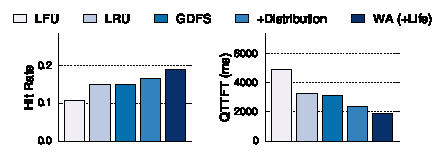
\includegraphics[width=1.0\linewidth,center]{./data/abl.pdf}  \\[3pt]
    \begin{minipage}{1\linewidth}
    \caption{\small{\emph{     
        An ablation study on Qwen2-7B with \#CPU Cache / HBM is 1.
    }}}
    \label{fig:cache-policy-abl}
    \end{minipage} \\[-5pt]
\end{figure}

\stitle{Ablation study. \,}
{\fig{fig:cache-policy-abl}} conducts an ablation study on the Qwen2-7B model on Trace A
with different policies. Other models share a similar trend.
First, we can see that using a distribution-based approach improves the
hit rate by 1\,\% (with technique \ding{192} in Table~\ref{tab:insights}).
Considering the short lifespan of {\kvcache} with the life regulator further
increases the hit rate by 2.4\,\% (\ding{194}).
Note that we omit describing the locality optimization \ding{193} as it is applied
to all the policies.

\iffalse
\subsection{Discussion}
\label{sec:discussion}
\stitle{Fairness Issue. \,}
Some readers may question the fairness of our policy—specifically, 
whether it might favor certain workload types while neglecting others. 
However, our probability-prediction-based policy retains 
specific workload types even if they do not occur frequently now, 
provided they have large probability to be reused within a future time window. 
In contrast, the cache space under LRU would be overwhelmed 
by transient one-time-use {kvcache} blocks which are unlikely to reappear.

\stitle{Security Issue. \,}
Some readers may worry that our caching policy could be 
exploited by malicious users through a large number of duplicate requests, 
thereby reducing the cache hit rate for other users. 
We consider this to be an orthogonal issue with respect to the caching policy itself. 
Before reaching the actual inference engine, 
user requests are also protected by defenses 
at both the application layer and gateway layer against such malicious attacks
in real-world LLM application.
\fi

\stitle{Discussion: fairness issue. \,}
Like all existing systems (and their policies),
a malicious client can monopolize prefix cache by sending a large volume of requests with long identical prefixes,
thus causing fairness issues.
Ensuring fairness is an orthogonal topic to cache policy
and can be addressed via a co-design of LLM serving strategies like FairRide~\cite{DBLP:conf/nsdi/PuLZGS16,DBLP:conf/osdi/0007CLZ0ZGS24}.